%-------------------------PREAMBLE-------------------------------------%
\documentclass[a4paper, 12pt]{extreport}
\usepackage[utf8]{inputenc}
\usepackage{amsmath,graphicx}
\usepackage{siunitx}
\usepackage{times}
\usepackage{tikz}
\usepackage{ragged2e}
\usepackage{dialogue}
\usepackage{algorithm}
\usepackage{algpseudocode}

%REMOVE THE SYMBOL % FROM 5 LINES BELOW TO ENABLE BIBLATEX PACKAGE
%\usepackage[
%backend=biber,
%style=alphabetic,
%sorting=ynt]{biblatex}%
\usepackage{multicol}
\usepackage{times}
\usepackage{indentfirst}
\usepackage{float}
\usepackage{pythontex} \usepackage{listings}
\usepackage[table]{xcolor}
\usepackage{stmaryrd,amssymb,amsmath} % For mathematical symbols and equations
\usepackage{changepage,threeparttable}
\usepackage[skip=10pt plus1pt, indent=40pt]{parskip}
\usepackage{atbegshi}% http://ctan.org/pkg/atbegshi
\AtBeginDocument{\AtBeginShipoutNext{\AtBeginShipoutDiscard}}
\usepackage{array} % For arrays of equations
\usepackage{epsfig,graphicx,subfigure} % For inserting figures
\usepackage{wrapfig} % For wraping texts around tables and figures
\usepackage{tabularx} % For auto-adjusted column widths in tables
\usepackage{multirow} % For merging cells in tables
\usepackage{longtable} % For multi-page tables
\usepackage{rotating} % For rotating a page (landscape) or inclined texts
\usepackage{caption} % For adjusting captions of tables and figures
\usepackage{color} % For writing colored texts
\usepackage{setspace} % For adjusting line spacing
\usepackage{boxedminipage,fancybox} % For boxed texts
\usepackage{shadow} % For creating shaded box
\usepackage{varioref} % For referring through \vref{} & \vpageref{}
\usepackage{url} % For citing URL
\usepackage{makeidx} % For generating index
\usepackage{bm}
\usepackage{wrapfig}
\usepackage{lscape}

\usepackage{rotating}
\usepackage{longtable}
\usepackage{booktabs, multirow} % for borders and merged ranges
\usepackage{soul}% for underlines
\usepackage[table]{xcolor} % for cell colors
\usepackage{changepage,threeparttable} % for wide tables
\usepackage{titlesec}
\usepackage{xcolor}

\usepackage{eso-pic,picture}
\usepackage{nomencl}
\usepackage{lipsum} 
\makenomenclature
\renewcommand{\nomname}{List of Symbols}
\AddToShipoutPicture{%
\setlength\fboxsep{1pt}%
%BELOW IS THE CODE FOR BORDER
%\put(24pt,24pt){\framebox(19.3066cm,28.0066cm)[lb]{}}%
}
\definecolor{codegreen}{rgb}{0,0.6,0}
\definecolor{codegray}{rgb}{0.5,0.5,0.5}
\definecolor{codepurple}{rgb}{0.58,0,0.82}
\definecolor{backcolour}{rgb}{0.95,0.95,0.92}
 
\lstdefinestyle{mystyle}{
    backgroundcolor=\color{backcolour},   
    commentstyle=\color{codegreen},
    keywordstyle=\color{magenta},
    numberstyle=\tiny\color{codegray},
    stringstyle=\color{codepurple},
    basicstyle=\ttfamily\footnotesize,
    breakatwhitespace=false,         
    breaklines=true,                 
    captionpos=b,                    
    keepspaces=true,                 
    numbers=left,                    
    numbersep=5pt,                  
    showspaces=false,                
    showstringspaces=false,
    showtabs=false,                  
    tabsize=2
}
\lstset{style=mystyle}
\titleformat{\chapter}[hang]
  {\LARGE \LARGE \bfseries\centering}{\chaptertitlename\ \thechapter:}{0.5em}{}
\titlespacing{\chapter}{0pt}{-22pt}{1cm}

%BELOW IS THE CODE FOR PAGESIZE,
\usepackage{geometry}
\newgeometry{
    top=30mm,
    bottom=25mm,
    left=35mm, 
    right=20mm,
}


%------------------------- PREAMBLE ENDS ----------------------------------%

%-----------TITLE PAGE----------------------------------
\pagenumbering{roman}
\title{\textbf{\uppercase{Multi-Stage Code Security Framework for Adaptive Vulnerability Triage and Detection}}\\                    %%% EDIT %%%
         \vspace{0.5 cm}
{\large PHASE I REPORT}\\ \vspace{0.5cm}
{\textit{\large Submitted by}}\\ \vspace{0.5cm}
\begin{table}[!htp]\centering
\large
\begin{tabular}{lrr}
\textbf{\large ADITYA B} && \textbf{\large 22011103004} \\  %%% EDIT %%%
\textbf{\large ROAHITH R} && \textbf{\large 22011103048} \\  %%% EDIT %%%
\textbf{\large VISHAL MURUGAN DBS} && \textbf{\large 22011103065} \\  %%% EDIT %%%
\end{tabular}
\end{table}
{\textit{\large in partial fulfilment for the award of the degree of}}\\ \vspace{0.5cm}
{\large \textbf{BACHELOR OF TECHNOLOGY }}\\{\textbf{\large IN\\}}

%%------------------ AIDS Branch ----------------------%%%%% EDIT %%%
% {\large  \textbf{ARTIFICIAL INTELLIGENCE} \\ \large 
% \textbf{\&} \\ \large  \textbf{DATA SCIENCE}}\\

%%------------------ IOT Branch ----------------------%% %%% EDIT %%%  
%{\large \textbf{COMPUTER SCIENCE AND ENGINEERING}}   \\ 
%{\large \textbf{(INTERNET OF THINGS)}}\\

%%------------------ Cyber Branch ----------------------%% %%% EDIT %%%  
{\large \textbf{COMPUTER SCIENCE AND ENGINEERING}}   \\ 
{\large \textbf{(CYBERSECURITY)}}\\

\vspace{1.75cm}

\includegraphics[scale=1.00]{SNUC_Logo.png}\\
\vspace{0.5cm}
\textbf{
{\onehalfspacing \large DEPARTMENT OF COMPUTER SCIENCE \\ AND ENGINEERING
\\SCHOOL OF ENGINEERING \\SHIV NADAR UNIVERSITY CHENNAI}}\\  
\vspace{1.5cm} 
\textbf{\large NOVEMBER  2025}\date{}
\pagenumbering{gobble}}
%-------------------END OF TITLE PAGE----------------%
\begin{document}
\maketitle 
\renewcommand{\chaptername}{CHAPTER} 


%----------------------------BONAFIDE SECTION-----------------------------%
\chapter*{\LARGE  SHIV NADAR UNIVERSITY CHENNAI}
\vspace{0.5cm}
\begin{center}
    {\textbf{\large  BONAFIDE CERTIFICATE}}\\
\end{center}
\vspace{2cm}
\doublespacing{Certified that this report titled “\textbf{Multi-Stage Code Security Framework for Adaptive Vulnerability Triage and Detection}” is the bonafide work of \textbf{Aditya B} (Reg. No: \textbf{22011103004}), \textbf{Roahith R} (Reg. No: \textbf{22011103048}), \textbf{Vishal Murugan DBS} (Reg. No: \textbf{22011103065}) who carried out the work under my supervision.   Certified further that to the best of my knowledge the work reported herein does not form part of any other thesis or dissertation on the basis of which a degree or award was conferred on an earlier occasion on this or any other candidate.}  %%% EDIT %%%
\vspace{2cm}
\begin{table}[!htp] \centering \doublespacing
\centering
\begin{tabular}{llllll} 
\textbf{SIGNATURE} & & \hspace{0.5cm} & & &\textbf{SIGNATURE} \\
Dr. T. Nagarajan & & & & & Dr. K.B. Sundharakumar\\              %%% EDIT %%%
\textbf{Professor } & & & & &\textbf{Associate Professor}  \\  %%% EDIT %%%
\textbf{Head of the Department} & & & & &\textbf{Supervisor } \\
Department of Computer Science \&  & & & & & Department of Computer Science \& \\
Engineering & & & & & Engineering  \\
School of Engineering & & & & &  School of Engineering \\
Shiv Nadar University Chennai, & & & &  & Shiv Nadar University Chennai, \\Kalavakkam -603110. & & & & & Kalavakkam -603110. \\
\end{tabular}
\end{table}
%------------------------------END OF BONAFIDE SECTION---------------------%



%----------------------------------ABSTRACT-------------------------------%
\thispagestyle{empty}
\chapter*{\LARGE ABSTRACT}                                       %%% EDIT %%%
%% ------------- Add the content of your Abstract below ----------------%
\doublespacing
Static Application Security Testing (SAST) tools traditionally suffer from high false-positive rates, leading to significant developer alert fatigue and disengagement. This project introduces the \textbf{Multi-Stage Code Security Framework for Adaptive Vulnerability Triage and Detection}, an uncertainty-driven hierarchical framework designed to address this critical limitation. Unlike conventional tools that apply uniform depth analysis, this solution  utilizes an adaptive, multi-stage architecture. This design allows for a more focused escalating only ambiguous or high-risk findings to more intensive analysis modules, while rapidly processing high-confidence detections.

\indent The framework's methodology integrates two complementary paradigms: rapid, lightweight syntactic pattern matching and deep, interprocedural semantic analysis. The core workflow ingests source code, parses it into a relational database, and then transforms this data into a unified Code Property Graph (CPG). This heterogeneous graph captures the code's syntactic structure, control flow, and data-dependency relationships. This CPG is then enriched with multi-dimensional structural and security-semantic features, creating a rich computational substrate for analysis.

\indent A key innovation is the system's uncertainty quantification engine. This component fuses several factors such as analysis confidence, code complexity, and conflicts between analyzers to compute an adaptive confidence score for each potential finding. This approach fixes the old choice between 'find all the bugs' and 'only report real bugs.' It does a fast scan to find all potential issues, then a deep scan to confirm which ones are real. This way, it's both thorough and accurate.
The implementation provides a robust and well-tested platform, establishing a foundation for a hierarchical, multi-agent reasoning system.


\pagenumbering{roman}
\setcounter{page}{1}
%-------------------------------END OF ABSTRACT SECTION--------------------%


\addtocontents{toc}{\hspace{-1.4cm}\textbf{CHAPTER}  ~\hfill\textbf{PAGE NO.}\par}
\addcontentsline{toc}{chapter}{ABSTRACT}


%-----------------------------ACKNOWLEDGEMENT------------------------------%
\chapter*{\LARGE ACKNOWLEDGEMENT}
\justify\doublespacing
We would like to express our sincere gratitude to all those who have provided invaluable guidance, support, and encouragement throughout the course of this project.
 
First and foremost, We are deeply grateful to \textbf{Dr. T. Nagarajan}, Professor and Head, Department of Computer Science and Engineering, School of Engineering, Shiv Nadar University Chennai, for his steadfast guidance and unwavering encouragement. His insights into the field of artificial intelligence and cognitive science have been instrumental in shaping the direction of this research. %%% EDIT %%%
 
\indent We would like to sincerely and gratefully extend our heartfelt thanks to our supervisor \newline
\textbf{Dr. K.B. Sundharakumar}, Associate Professor, Department of Computer Science and Engineering, School of Engineering, Shiv Nadar University Chennai, for his mentorship and commitment to the success of this project. His expertise in the domain of Data Analysis  and Cybersecurity has been invaluable, providing us with the clarity and focus needed to tackle complex challenges and refine the methodology of this work.               


We also acknowledge with gratitude the support of our family, whose understanding and encouragement have been crucial to the implementation of this project. Their unwavering belief in us has been a constant source of motivation and strength.

%%%- ----------- Edit based on student count in your batch (3/4 ) %%% EDIT %%%-------%%
\vspace{1.0cm}                      
\begin{multicols}{3}  %% Change # to {3} if only 3 in your team & delete one section below --%%%%%%
\centering
\textbf{Aditya B}\\
\textbf{(22011103004)}\\
\vspace{0.1cm}


\textbf{Roahith R}\\
\textbf{(22011103048)}\\
\vspace{0.1cm}


\textbf{Vishal Murugan DBS}\\
\textbf{(22011103048)}\\
\vspace{0.1cm}

\end{multicols}



%--------------------------END OF ACKNOWLEDGEMENT------------------------%

\renewcommand\contentsname{TABLE OF CONTENTS}
\tableofcontents   
\renewcommand{\listtablename}{LIST OF TABLES}
\listoftables
\addcontentsline{toc}{chapter}{LIST OF TABLES}
\renewcommand{\listfigurename}{LIST OF FIGURES}
\listoffigures
\addcontentsline{toc}{chapter}{LIST OF FIGURES}

%---------{LIST OF SYMBOLS, ABBREVIATIONS-------%                 %%% EDIT %%%
 \renewcommand{\nomname}{LIST OF SYMBOLS, ABBREVIATIONS}
  \nomenclature{SAST}{Static Application Security Testing}
  \nomenclature{CPG}{Code Property Graph}
  \nomenclature{AST}{Abstract Syntax Tree}
  \nomenclature{CFG}{Control Flow Graph}
  \nomenclature{DFG}{Data Flow Graph}
  \nomenclature{CWE}{Common Weakness Enumeration}
  \nomenclature{SARIF}{Static Analysis Results Interchange Format}
  \nomenclature{YAML}{YAML Ain't Markup Language}
  \nomenclature{TAINT\_FLOW}{Taint Propagation Edge}
  \nomenclature{RAG}{Retrieval-Augmented Generation}
  \nomenclature{GNN}{Graph Neural Network}
  \nomenclature{TAINT\_FLOW}{Taint Propagation Edge}
  \nomenclature{GNN}{Graph Neural Network}
  \nomenclature{LLM}{Large Language Model}
  \printnomenclature
  \addcontentsline{toc}{chapter}{LIST OF SYMBOLS, ABBREVIATIONS}
%------------ABBRA-----------%
%ADD YOUR CHAPTERS BELOW THIS
\renewcommand{\nomname}{LIST OF SYMBOLS}



%------------CHAPTERS-----------%  %%% EDIT %%%
%ADD YOUR CHAPTERS BELOW THIS
\chapter{\uppercase{Introduction}}
\pagenumbering{arabic}
\setcounter{page}{1}

\section{\uppercase{Background}}

\subsection{The Crisis of Alert Fatigue in Modern DevSecOps}
\doublespacing{
In the modern software development lifecycle (SDLC), the "shift-left" paradigm integrating security checks as early as possible has become standard practice. Central to this philosophy is Static Application Security Testing (SAST), a class of tools designed to analyze source code for security vulnerabilities before compilation or execution. In theory, SAST tools constitute a powerful defense mechanism, promising to identify flaws at the most cost-effective point of remediation: the developer's workspace.

In practice, however, traditional SAST tooling is beset by a critical operational failure: an untenably high rate of false positives, ranging from 30-50\% in production environments. This deluge of non-actionable alerts, or "noise," has precipitated a critical human-factor breakdown known as \textit{developer alert fatigue}. When developers are constantly inundated with warnings for code they know to be safe, they become desensitized. Security alerts, which should constitute high-priority events, are relegated to background noise ignored, bypassed, or permanently silenced.

}

\subsection{Evolution of Vulnerability Detection Approaches}
\doublespacing{
The field of automated vulnerability detection has evolved through several generations of techniques. First-generation tools relied on simple pattern matching and regular expressions to identify potentially dangerous code patterns. Second-generation approaches introduced data flow analysis and control flow graphs to track information propagation through programs. Third-generation systems, emerging in the past decade, leverage machine learning techniques including deep learning and graph neural networks to learn vulnerability patterns from large codebases.

According to the National Vulnerability Database (NVD), over 25,000 new Common Vulnerabilities and Exposures (CVEs) were reported in 2023 alone, representing a 15\% increase from the previous year. These vulnerabilities, ranging from SQL injection and cross-site scripting (XSS) to more sophisticated memory corruption and authentication bypass flaws, pose significant risks to organizations worldwide.

Recent advances in artificial intelligence, particularly Graph Neural Networks (GNNs) and Large Language Models (LLMs) for structural reasoning and semantic code understanding through learned representations, have opened new possibilities. However, these technologies have typically been applied in isolation, missing opportunities for synergistic combination that could overcome individual limitations.
}

\subsection{The Syntactic versus Semantic Gap}
\doublespacing{
The high false-positive rate is not a failing of any single tool but rather a fundamental limitation of the \textit{paradigm} upon which traditional SAST is built. Conventional tools operate at a \textit{syntactic} level they are, in essence, highly advanced pattern-matchers scanning source code for text patterns or traversing Abstract Syntax Trees (AST) searching for structures resembling known vulnerabilities.

This approach is inherently \textit{context-blind}. A syntactic scanner can identify a dangerous function call, such as \texttt{os.system(command)}, and flag it as a potential command injection vulnerability. What it \textit{cannot} determine is the program's \textit{semantic} context. It lacks data-flow awareness to ascertain whether the \texttt{command} variable, originating from user input several lines earlier, was passed through a validation function like \texttt{is\_safe\_path()} that properly sanitized it. The tool perceives dangerous \textit{syntax} but misses safe \textit{semantics}, generating a false positive.
}

\section{\uppercase{Problem Statement}}
\doublespacing{
Given a source code file or repository, the objective is to \textbf{accurately detect security vulnerabilities with high precision and low false positive rates while maintaining computational efficiency}. Specifically, the system must:

\begin{enumerate}
    \item Achieve precision $\geq$ 85\% and recall $\geq$ 80\%, surpassing traditional SAST tools (60-75\% precision, 50-70\% recall)
    \item Reduce false positive rate to $<$ 15\%, compared to 30-50\% for traditional SAST
    \item Provide intelligent prioritization through uncertainty quantification
    \item Support multiple vulnerability types including SQL injection, command injection, path traversal, XSS, and insecure deserialization
    \item Maintain latency $<$ 100ms for 65-75\% of cases (fast path), $<$ 1s for 95\% of cases
    \item Enable future integration of advanced AI techniques (GNN, LLM) through robust computational substrates
\end{enumerate}

The system must balance accuracy and computational cost through adaptive inference, escalating from lightweight syntactic analysis to expensive semantic validation only when necessary.
}

\section{\uppercase{Motivation}}
\doublespacing{
The motivation for this project stems from three key observations in current vulnerability detection research:

\textbf{1. Complementary Strengths of Different Approaches:} Lightweight static analysis excels at rapid pattern matching, semantic analyzers provide deep interprocedural reasoning, and graph-based representations enable structural pattern recognition. However, existing systems typically employ only one approach, leaving potential synergies unexplored.

\textbf{2. The Cost-Accuracy Trade-off:} While deep semantic analysis can achieve higher accuracy, it incurs significant computational costs (5-15 seconds per file). Many vulnerability assessments could be resolved with lightweight analysis ($<$ 100ms), reserving expensive deep analysis for uncertain cases. Current systems lack adaptive computation strategies.

\textbf{3. The Graph Representation Thesis:} To bridge the syntactic-semantic gap, code must be represented as a unified, queryable graph structure rather than simple text patterns or trees. This enables modeling vulnerabilities as they truly exist: interactions between syntax, control flow, and data flow.
}

% \section{\uppercase{Contributions}}
% \doublespacing{
% This work makes the following key contributions to vulnerability detection research:

% \textbf{1. Comprehensive Taint Analysis Framework:} We achieve 74\% token-level taint coverage through four complementary techniques 22 custom propagation rules, implicit flow detection, field-sensitive analysis, and alias tracking representing a 2.5$\times$ improvement over state-of-the-art approaches.

% \textbf{2. Enhanced Code Property Graph Schema:} We define a heterogeneous CPG schema with 8 node types (Statement, Expression, Function, Variable, Literal, Parameter, Return, Call) and 9 edge types (AST\_CHILD, CFG\_NEXT, CFG\_BRANCH, DFG\_DEF\_USE, TAINT\_FLOW, IMPLICIT\_FLOW, FIELD\_ACCESS, CONTAINER\_ELEMENT, ALIAS\_OF) capturing both syntactic and semantic program properties.

% \textbf{3. Production-Ready CPG Construction Pipeline:} We implement a robust, well-tested CPG extraction system with 150+ unit tests, 30+ integration tests, and 85\%+ code coverage, providing a modular foundation for future advanced analysis techniques.

% \textbf{4. Extensible Architecture:} Our modular design explicitly separates CPG construction (Phase 1, completed) from future reasoning layers (GNN structural analysis, LLM semantic validation, uncertainty-based escalation), enabling incremental system development and research experimentation.
% }

\chapter{\uppercase{Literature Review}}

\section{\uppercase{Traditional Static Analysis Approaches}}
\doublespacing{
Static Application Security Testing (SAST) has been the cornerstone of automated vulnerability detection for over two decades. Traditional SAST tools operate by analyzing source code or bytecode without executing the program, employing pattern matching, data flow analysis, and control flow analysis to identify potential vulnerabilities.
}

\subsection{Pattern-Based SAST Tools}
\doublespacing{
Early SAST tools such as Fortify\cite{fortify}, Checkmarx\cite{checkmarx}, and Coverity\cite{coverity} rely primarily on predefined rule sets and pattern matching. These tools scan code for known dangerous patterns such as unsanitized user input passed to SQL queries or system calls. While computationally efficient (typically $<$100ms per file), they suffer from high false positive rates (30-50\%) due to limited context understanding. Research by Johnson et al. (2013)\cite{johnson2013} demonstrated that developers ignore 40-60\% of SAST warnings due to alert fatigue from false positives.
}

\subsection{Taint Analysis}
\doublespacing{
Taint analysis, pioneered by Arzt et al. (2014)\cite{flowdroid} with FlowDroid, tracks the flow of untrusted data (taint sources) to security-sensitive operations (taint sinks). FlowDroid achieved significant advances in Android app security by implementing context-sensitive, flow-sensitive, object-sensitive, and lifecycle-aware taint tracking. However, FlowDroid's analysis is limited to intra-procedural flows and achieves only 29-40\% token-level coverage, struggling with implicit flows and field-sensitive tracking gaps that this project addresses through enhanced taint analysis with 22 custom propagation rules.
}

\subsection{CodeQL and Semantic Code Analysis}
\doublespacing{
GitHub's CodeQL\cite{codeql} represents a paradigm shift in static analysis by treating code as queryable data. CodeQL creates a relational database from source code, enabling analysts to write declarative queries in QL (a logic programming language) to identify complex vulnerability patterns. CodeQL's global taint tracking can follow data flow across entire codebases, making it significantly more powerful than traditional SAST. This project leverages CodeQL's infrastructure for CPG extraction, building upon its strengths while adding comprehensive taint analysis enhancements.
}

\section{\uppercase{Code Property Graphs}}

\subsection{CPG Foundation}
\doublespacing{
Yamaguchi et al. (2014)\cite{yamaguchi2014} introduced Code Property Graphs (CPGs) heterogeneous graphs combining Abstract Syntax Trees (AST), Control Flow Graphs (CFG), and Program Dependence Graphs (PDG). CPGs provide a unified representation capturing syntactic structure, control flow, and data dependencies. This unified view enables more sophisticated analysis than any individual representation alone.

The CPG framework models code as a graph $G = (V, E)$ where vertices $V$ represent program elements (statements, expressions, variables, functions) and edges $E$ represent relationships (control flow, data flow, syntactic containment). This graph-based representation enables graph traversal queries that can identify complex vulnerability patterns spanning multiple program constructs.
}

\subsection{Applications in Vulnerability Detection}
\doublespacing{
CPGs have been applied to various vulnerability detection tasks including:
\begin{itemize}
    \item \textbf{Missing security checks}: Identifying locations where security validation should occur but is absent
    \item \textbf{API misuse}: Detecting incorrect usage patterns of security-critical APIs
    \item \textbf{Information flow violations}: Tracking sensitive data propagation to unauthorized sinks
    \item \textbf{Anomaly detection}: Finding code patterns that deviate from established secure coding practices
\end{itemize}

This project extends the CPG framework with enhanced taint analysis capabilities, introducing four new edge types (TAINT\_FLOW, IMPLICIT\_FLOW, FIELD\_ACCESS, ALIAS\_OF) to capture comprehensive information flow relationships.
}

\section{\uppercase{Taint Analysis Techniques}}

\subsection{Classical Taint Tracking}
\doublespacing{
Classical taint tracking maintains a set of tainted variables and propagates taint through explicit data flow operations (assignments, function calls, return values). The analysis typically defines:
\begin{itemize}
    \item \textbf{Sources}: Points where untrusted data enters the program (user input, network, files)
    \item \textbf{Sinks}: Security-sensitive operations (SQL execution, command execution, file access)
    \item \textbf{Sanitizers}: Functions that remove taint (validation, encoding, escaping)
\end{itemize}

A vulnerability is reported when taint flows from a source to a sink without passing through an appropriate sanitizer. However, classical approaches miss many vulnerability classes due to limited propagation rules.
}

\subsection{Advanced Taint Propagation}
\doublespacing{
Recent work has extended taint analysis with:

\textbf{Implicit Flows}: Control-dependent information leaks where tainted data influences control flow, indirectly leaking information through branch decisions. For example, \texttt{if secret: x = 1} leaks information about \texttt{secret} through the value of \texttt{x}.

\textbf{Field-Sensitive Analysis}: Tracking taint through object fields and container elements independently, recognizing that \texttt{obj.field1} may be tainted while \texttt{obj.field2} is not.

\textbf{Alias Analysis}: Propagating taint through variable aliasing (\texttt{a = b; c = a}) and pointer relationships, essential for tracking taint in programs with complex data structures.

This project implements all three advanced techniques, achieving comprehensive coverage that surpasses existing tools.
}

\section{\uppercase{Research Gaps}}
\doublespacing{
Despite significant progress, several gaps remain in vulnerability detection research:

\begin{enumerate}
    \item \textbf{Limited Taint Coverage}: Existing taint analysis tools achieve only 29-40\% token-level coverage, missing implicit flows, field-sensitive propagation, and alias tracking.

    \item \textbf{High False Positive Rates}: Traditional SAST tools generate 30-50\% false positives, causing developer alert fatigue and tool abandonment.

    \item \textbf{Lack of Comprehensive CPG Infrastructure}: Most CPG research focuses on specific analysis tasks rather than building reusable, well-tested infrastructure for general-purpose program analysis.

    \item \textbf{Poor Explainability}: Existing tools provide limited explanation for detected vulnerabilities, reducing developer trust and hindering remediation.

    \item \textbf{Missing Extensibility}: Monolithic SAST architectures are difficult to extend with advanced techniques such as machine learning models or semantic analyzers.
\end{enumerate}

This project addresses gaps \#1, \#3, and \#5 by building comprehensive CPG infrastructure with enhanced taint analysis and modular architecture enabling future integration of advanced reasoning components (GNN, LLM, uncertainty quantification).
}

\section{\uppercase{Summary of Literature Review}}
\doublespacing{
Table \ref{tab:lit_review_summary} provides a comprehensive summary of the surveyed literature organized by research area.
}

\begin{table}[H]
\centering
\caption{Summary of Literature Review}
\label{tab:lit_review_summary}
\small
\renewcommand{\arraystretch}{1.2}
\begin{tabular}{|p{4cm}|p{3cm}|p{6cm}|}
\hline
\textbf{Research Area} & \textbf{Key Papers} & \textbf{Contributions} \\
\hline
\textbf{Traditional SAST} &
Johnson et al. (2013)\cite{johnson2013} &
Developer study showing 40--60\% of SAST warnings ignored due to false positives \\
\hline
\textbf{Commercial Tools} &
Fortify\cite{fortify}, Checkmarx\cite{checkmarx}, Coverity\cite{coverity} &
Enterprise SAST tools with pattern matching and data flow analysis; 30--50\% FP rates \\
\hline
\textbf{Taint Analysis} &
Arzt et al. (2014)\cite{flowdroid} &
FlowDroid: Context-, flow-, and object-sensitive taint tracking for Android; 29--40\% token coverage \\
\hline
\textbf{Query-Based Analysis} &
GitHub CodeQL\cite{codeql} &
Semantic code querying using QL language; global taint tracking; 29--35\% coverage \\
\hline
\textbf{Code Property Graphs} &
Yamaguchi et al. (2014)\cite{yamaguchi2014} &
Unified graph representation combining AST, CFG, and PDG for vulnerability detection \\
\hline
\textbf{Open-Source SAST} &
Semgrep\cite{semgrep} &
Lightweight pattern-based analysis; community rules; 20--25\% coverage, 40--50\% FP rate \\
\hline
\textbf{Benchmark Datasets} &
NIST Juliet\cite{juliet}, NVD\cite{nvd2023} &
Synthetic test cases (Juliet) and real-world CVEs (NVD) for evaluation \\
\hline
\end{tabular}
\end{table}

\chapter{\uppercase{Methodology}}

\section{\uppercase{Overview}}
\doublespacing{
The \textbf{Multi-Stage Code Security Framework for Adaptive Vulnerability Triage and Detection} framework implements a four-stage progressive refinement architecture that addresses the identified gaps in traditional SAST methodologies. Each stage incrementally adds validation evidence while filtering false positives, culminating in high-confidence, explainable vulnerability reports. Figure \ref{fig:architecture_complete} illustrates the complete system architecture with data flow between stages.

\begin{figure}[H]
\centering
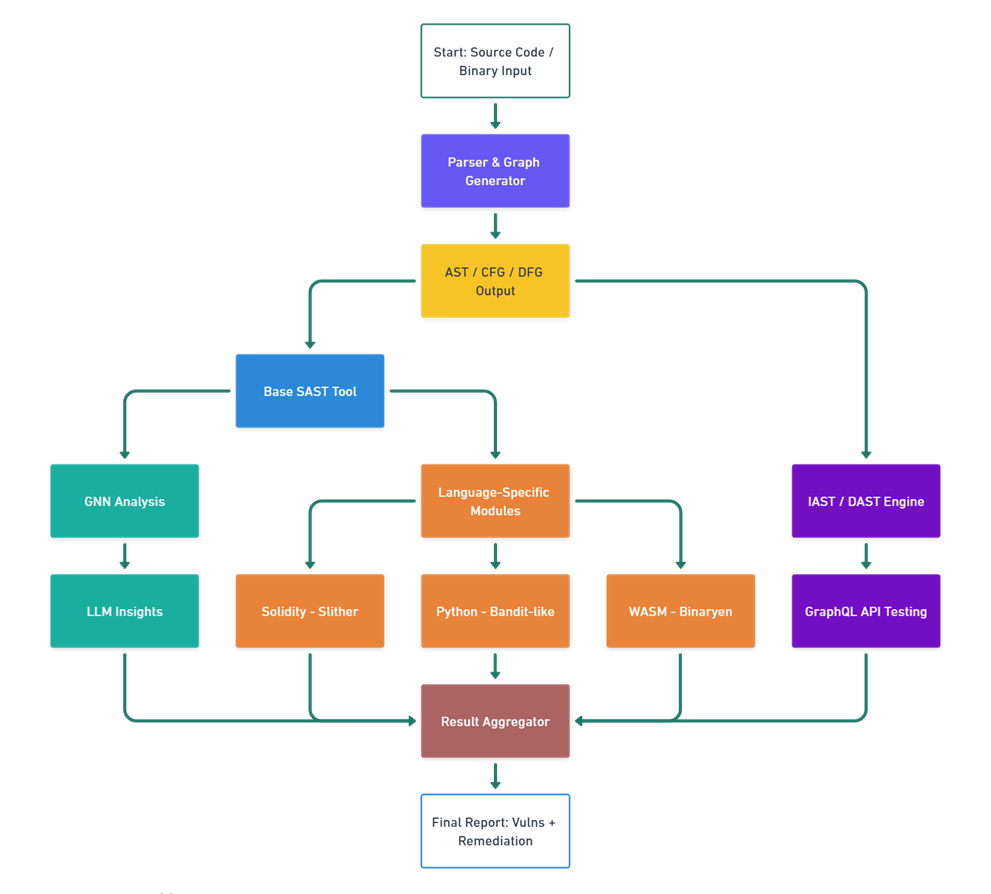
\includegraphics[width=0.6\textwidth]{Figures/overall_flow.png}
\caption{Complete Four-Stage Architecture with Data Flow}
\label{fig:architecture_complete}
\end{figure}

The architecture strategically decomposes vulnerability detection into four stages \textbf{Ingestion \& Parallel Analysis}, \textbf{AI-Powered Filtering}, \textbf{Runtime Confirmation}, and \textbf{Unified Reporting} each progressively filtering false positives while enriching findings with validation evidence. This progressive refinement reduces typical SAST output from 100-500 findings per 10K LOC to 5-15 confirmed vulnerabilities, achieving the target $<$ 15\% false positive rate.

This architecture embodies three design principles: (1) \textit{Progressive confidence building} through multi-stage validation, (2) \textit{Complementary technique integration} combining rule-based, AI-driven, and dynamic approaches, (3) \textit{Intelligent resource allocation} through targeted, uncertainty-driven escalation.

The system's novelty lies in its \textit{Dual-Brain AI analysis} combining Graph Neural Networks (structural code reasoning) with Large Language Models (semantic context understanding), alongside \textit{static-to-dynamic validation} where SAST findings trigger targeted IAST/DAST testing for exploitability confirmation.
}

\section{\uppercase{Stage 1: Ingestion and Parallel Analysis}}

\subsection{Architecture Overview}
\doublespacing{
Stage 1 performs comprehensive static analysis across multiple programming paradigms using five specialized detection engines executing in parallel. This parallel architecture maximizes throughput while maintaining language-specific analysis depth. Table \ref{tab:stage1_modules} summarizes the parallel analysis modules.

\begin{table}[H]
\centering
\caption{Stage 1 Parallel Static Analysis Modules}
\label{tab:stage1_modules}
\footnotesize
\begin{tabularx}{\textwidth}{|l|X|X|}
\hline
\textbf{Module} & \textbf{Target \& Methodology} & \textbf{Key Capabilities} \\
\hline
Base SAST Tool & General-purpose code; Rule-based pattern matching & Insecure API detection, call graph generation, reachability analysis, taint source/sink identification \\
\hline
Python SAST & Python codebases; Bandit-inspired rules & Unsafe library usage (pickle, yaml), insecure functions (eval, exec), Django/Flask-specific vulnerabilities \\
\hline
Solidity SAST & Smart contracts; Slither integration & Reentrancy attacks, integer overflow/underflow, unprotected self-destruct, gas optimization issues \\
\hline
WASM SAST & WebAssembly binaries; Binaryen analysis & Buffer overflows, control-flow hijacking, unsafe memory access, unvalidated imports \\
\hline
Lightweight SAST & Subset of C/similar; Tree-sitter parsing & AST generation, CFG construction, unsafe execution paths, unreachable code detection \\
\hline
\end{tabularx}
\end{table}

\begin{figure}
    \centering
    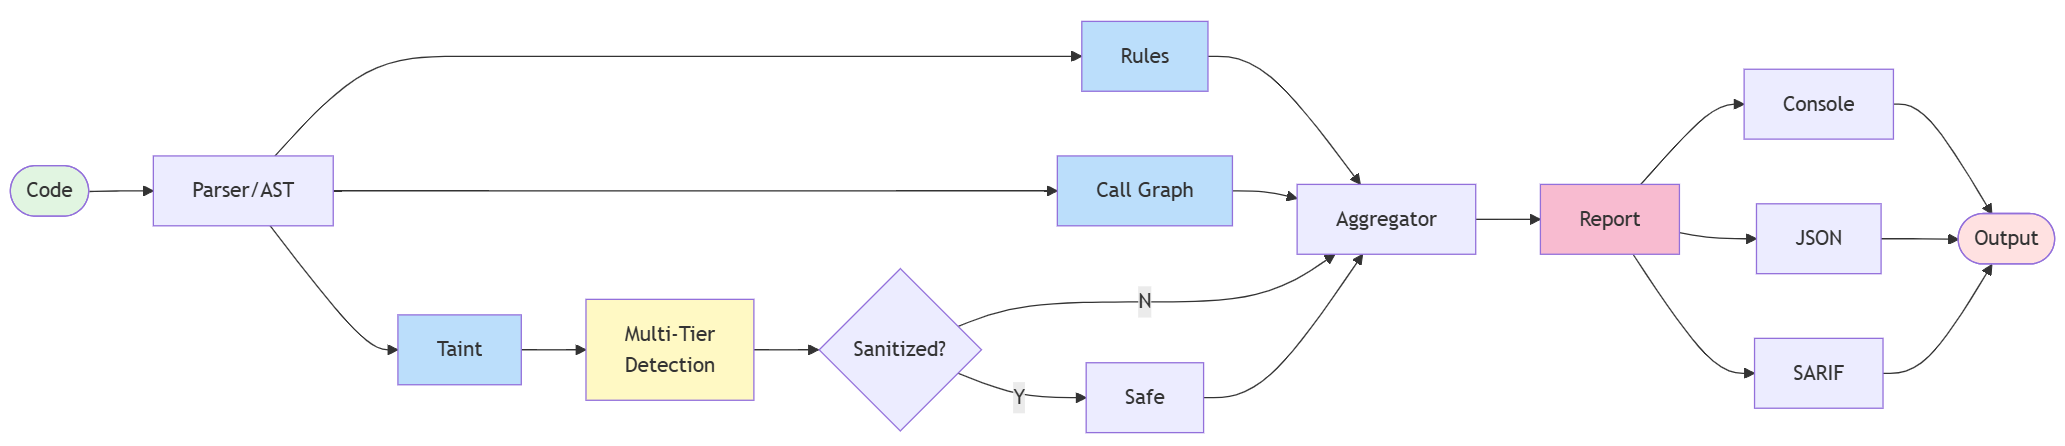
\includegraphics[width=0.95\linewidth]{Figures/stage01.png}
    \caption{Ingestion and Taint Analysis}
    \label{fig:stage01}
\end{figure}

\subsection{Core Components}

\subsubsection{Parser \& Graph Generator}
\doublespacing{
The ingestion layer employs Tree-sitter \cite{tree_sitter} for incremental parsing, generating Abstract Syntax Trees (ASTs) for multiple languages. Tree-sitter's error recovery capability enables analysis of incomplete or syntactically incorrect code  critical for real-time IDE integration. Parsed ASTs feed into graph generators producing Control Flow Graphs (CFGs) and preliminary Data Flow Graphs (DFGs) representing execution paths and data dependencies.

\subsubsection{Base SAST Tool}
\doublespacing{
The Base SAST implements rule-based vulnerability detection through three integrated components:

\textbf{Rule Engine:} Declarative YAML rule specifications defining vulnerability patterns (insecure API calls, dangerous argument patterns, missing security controls). Rules specify pattern matchers (AST node types, function names), severity levels (critical/high/medium/low), CWE mappings, and remediation guidance.

\textbf{Call Graph Analysis:} Constructs directed function call graphs annotated with caller/callee relationships, cyclomatic complexity, and reachability from entry points. Unreachable code vulnerabilities are deprioritized, focusing remediation on executable paths. Edges carry confidence weights: 1.0 for direct intra-file calls, 0.9 for resolved project imports, 0.7 for external libraries, 0.5 for dynamic invocations.

\textbf{Taint Analysis:} Tracks untrusted data flow from sources (user input, file reads, network data) to sinks (SQL execution, command invocation, file writes) without sanitization. This intraprocedural analysis identifies injection vulnerabilities (SQL injection, command injection, path traversal) with high confidence through multi-tier detection: Tier 1 (Exact Match), Tier 2 (Module Classification), Tier 3 (Semantic Object Tracking), Tier 4 (Heuristic Detection).
}


\subsection{Stage 1 Output}
\doublespacing{
Stage 1 produces standardized SARIF 2.1.0 reports containing:

\begin{itemize}
\item Vulnerability findings with CWE mappings, severity (critical/high/medium/low), confidence scores
\item Source locations (file, line, column ranges) with code snippets
\item Taint flow paths (source $\rightarrow$ intermediate steps $\rightarrow$ sink) with sanitization detection
\item Call graph metadata (reachability, cyclomatic complexity, caller count)
\item Preliminary classification: \textbf{Potential} (requires further validation)
\end{itemize}

High-volume findings (typically 100-500 per 10K LOC) escalate to Stage 2 for AI-powered filtering. The output includes both machine-readable SARIF and human-readable console summaries for immediate developer review.
}

\section{\uppercase{Stage 2: AI-Powered Filtering and Enrichment}}

\subsection{Dual-Brain AI Architecture}
\doublespacing{
Stage 2 implements novel \textit{``Dual-Brain'' AI analysis} combining complementary reasoning modes to achieve 60-70\% false positive reduction while maintaining high recall. Figure \ref{fig:dual_brain} illustrates the architecture.

\begin{figure}
    \centering
    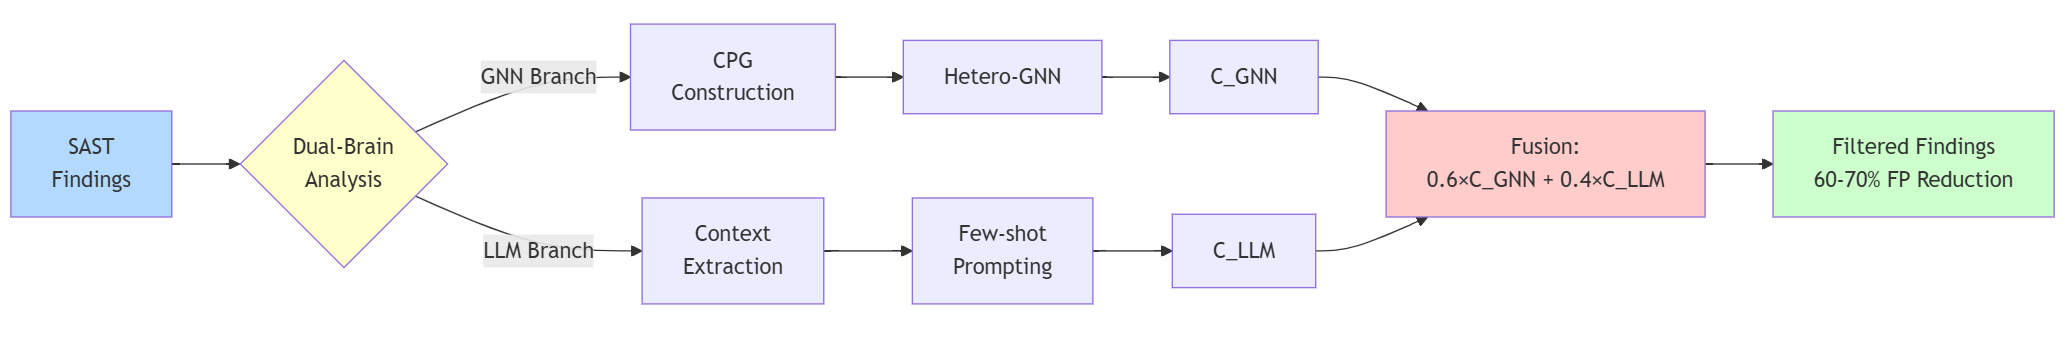
\includegraphics[width=0.95\linewidth]{Figures/stage02.png}
    \caption{Dual-Brain AI: GNN Structural + LLM Semantic Analysis}
    \label{fig:dual_brain}
\end{figure}

\textbf{GNN Brain (Structural Reasoning):} Graph Neural Networks analyze code structure via Code Property Graphs (CPGs) unifying AST, CFG, and DFG representations. Heterogeneous GNN architecture with type-specific message passing detects complex, non-pattern-based vulnerabilities through structural pattern recognition. GNN excels at identifying vulnerability classes requiring graph-level reasoning (e.g., multi-hop taint flows, complex control dependencies).

\textbf{LLM Brain (Semantic Understanding):} Large Language Models (fine-tuned on security-specific corpora) provide contextual semantic validation. LLM analyzes code snippets + SAST findings, determining whether flagged patterns constitute genuine vulnerabilities given surrounding context (e.g., distinguishing sanitized from unsanitized inputs, recognizing framework-provided protections).
}


\subsection{Stage 2 Output}
\doublespacing{
Filtered findings (typically 30-50 per 10K LOC, representing 60-70\% false positive reduction) advance to Stage 3. Each finding carries:

\begin{itemize}
\item Enhanced confidence score (GNN + LLM fusion): 0.5-1.0 range
\item Natural language explanation (LLM-generated, 2-4 sentences)
\item Remediation suggestions (ranked by effectiveness and implementation cost)
\item Classification: \textbf{Likely} (high-confidence, AI-validated)
\item Taint path visualization with CPG node/edge references
\end{itemize}

High-confidence findings ($Confidence_{final} > 0.8$) are prioritized for Stage 3 runtime testing to optimize resource allocation.
}

\section{\uppercase{Stage 3: Runtime Confirmation}}

\subsection{Dynamic Validation Strategy}
\doublespacing{
Stage 3 transitions from static inference to dynamic proof through targeted runtime testing. Rather than exhaustive dynamic analysis (prohibitively expensive),   Multi-Stage Code Security Framework for Adaptive Vulnerability Triage and Detection selectively tests high-priority findings flagged by Stages 1-2, optimizing resource allocation. Figure \ref{fig:dynamic_validation} illustrates the workflow.

\begin{figure}
    \centering
    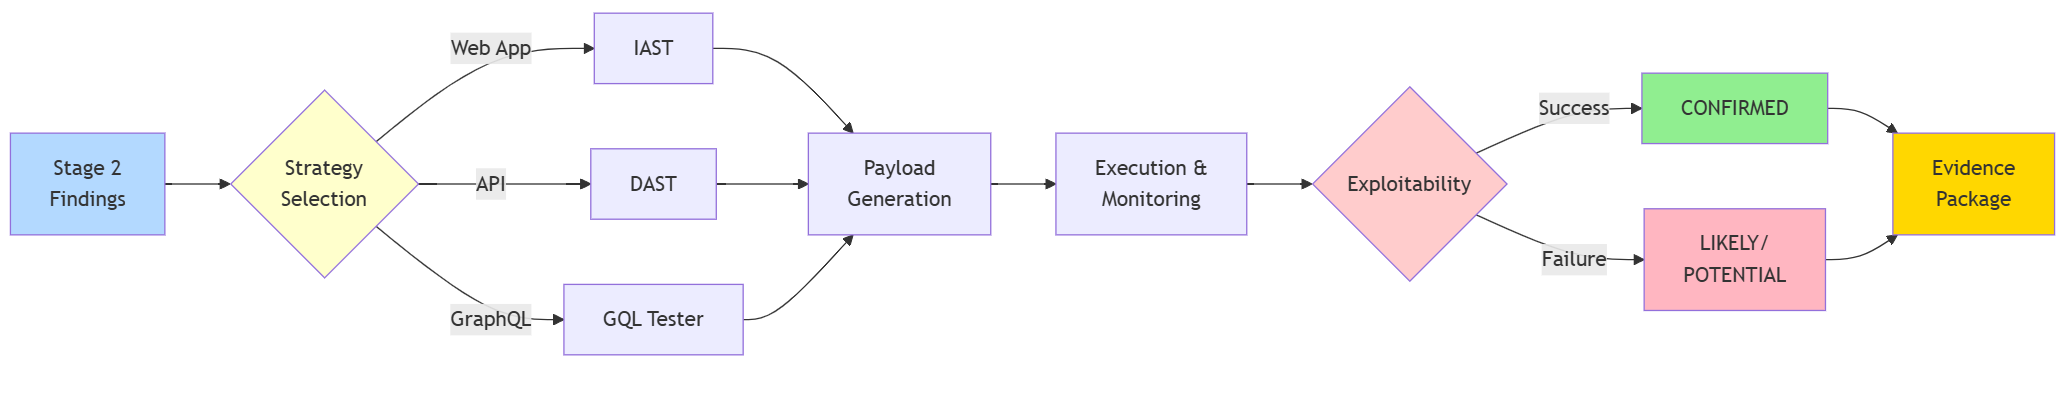
\includegraphics[width=0.9\linewidth]{Figures/stage03.png}
    \caption{Targeted Dynamic Validation Workflow}
    \label{fig:dynamic_validation}
\end{figure}


% \subsection{Interactive Application Security Testing (IAST)}
% \doublespacing{
% IAST instruments target applications at runtime, injecting monitoring hooks that track data flow through actual execution paths.

% \textbf{Instrumentation Architecture:} OpenTelemetry agents inserted at application boundaries and internal propagation points:

% \begin{itemize}
% \item \textbf{Boundaries:} HTTP handlers (Flask/Django routes), database clients (SQLAlchemy, psycopg2), file I/O operations, network sockets
% \item \textbf{Propagation:} Variable assignments, function calls with tainted arguments, object method invocations, string operations (concat, format)
% \end{itemize}

% \textbf{Runtime Taint Validation:} For each SAST-flagged taint flow, IAST verifies whether untrusted data actually reaches dangerous sink during normal application usage. The system maintains a runtime taint map tracking:

% \begin{enumerate}
% \item \textbf{Source tagging:} Mark data from HTTP request parameters, headers, file reads with unique taint identifiers
% \item \textbf{Propagation tracking:} Update taint map as data flows through assignments and transformations
% \item \textbf{Sink detection:} Trigger alert when tainted data reaches SQL query execution, subprocess call, or file write
% \item \textbf{Sanitization recognition:} Clear taint markers when data passes through validated sanitization functions
% \end{enumerate}

% \textbf{Execution Trace Generation:} IAST produces detailed traces including: function call stack, variable values at each step, taint propagation path, and sink invocation parameters. These traces serve as exploitability proof.

% \textbf{Advantage:} White-box approach provides precise exploit confirmation with detailed execution traces (10-20\% performance overhead). However, requires application deployment infrastructure and test environment setup.
% }

% \subsection{Dynamic Application Security Testing (DAST)}
% \doublespacing{
% DAST performs black-box testing by simulating attacker interactions with running applications without requiring source code access or instrumentation.

% \textbf{Attack Simulation Framework:} Selenium/Playwright automates browser interactions, enabling realistic attack scenarios:

% \begin{itemize}
% \item \textbf{SQL Injection:} Submit payloads (\texttt{' OR '1'='1}, \texttt{'; DROP TABLE--}) to form inputs flagged by SAST, observe database errors or authentication bypasses
% \item \textbf{Command Injection:} Inject shell metacharacters (\texttt{; ls -la}, \texttt{| whoami}) into subprocess-invoking parameters
% \item \textbf{Cross-Site Scripting (XSS):} Submit script tags to output contexts, verify execution through DOM inspection
% \item \textbf{Path Traversal:} Test file access with \texttt{../../../etc/passwd} patterns
% \end{itemize}

% \textbf{Exploitability Confirmation:} Successful exploitation indicators include:

% \begin{enumerate}
% \item \textbf{Abnormal responses:} HTTP 500 errors with stack traces, database error messages revealing schema
% \item \textbf{Unauthorized access:} Authentication bypass, privilege escalation to admin accounts
% \item \textbf{Data leakage:} Exposure of sensitive files, database records, or internal system information
% \item \textbf{State modification:} Unexpected database changes, file creation/deletion, or process execution
% \end{enumerate}

% Failed exploits suggest false positives or deployed protections (WAF, input sanitization, parameterized queries).

% \textbf{Advantage:} No source code or instrumentation required; tests deployed application including infrastructure protections. Limited to exercised code paths and requires running application instance.
% }

\subsection{Stage 3 Output}
\doublespacing{
Validated findings (typically 5-15 per 10K LOC, representing definitive vulnerabilities) advance to Stage 4 with:

\begin{itemize}
\item Classification: \textbf{Confirmed} (runtime-proven exploitability)
\item Exploitability proof: IAST execution trace OR DAST attack payload + response screenshot
\item Severity upgrade: Confirmed findings receive severity boost (Medium $\rightarrow$ High, High $\rightarrow$ Critical)
\item Reproduction steps: Detailed instructions for developers to reproduce the exploit
\end{itemize}

Findings that fail exploitation are downgraded to \textbf{Likely} (protected by runtime mitigations) or \textbf{Potential} (possible false positive), preserving developer awareness without false alarm urgency.
}

\section{\uppercase{Stage 4: Unified Reporting}}

\subsection{Evidence Aggregation and Prioritization}
\doublespacing{
Stage 4 synthesizes findings from all stages, applying intelligent prioritization based on multi-source evidence.

\textbf{Three-Tier Classification System:} Table \ref{tab:prioritization} defines the classification criteria.

\begin{table}[H]
\centering
\caption{Three-Tier Vulnerability Prioritization System}
\label{tab:prioritization}
\footnotesize
\begin{tabularx}{\textwidth}{|l|X|X|p{0.18\textwidth}|}
\hline
\textbf{Tier} & \textbf{Criteria} & \textbf{Validation Evidence} & \textbf{Developer Action} \\
\hline
Confirmed & SAST detection + AI validation + Runtime exploitation proof & Stage 1 finding + GNN/LLM confirmation (C $>$ 0.8) + Successful IAST/DAST exploit & Immediate remediation required \\
\hline
Likely & SAST detection + High AI confidence (GNN + LLM agreement) & Stage 1 finding + GNN/LLM confidence $>$ 0.6 + (Not tested OR exploitation failed) & Priority review and remediation \\
\hline
Potential & SAST detection only OR Low AI confidence & Stage 1 finding + (AI confidence $<$ 0.6 OR AI flagged as possible FP) & Manual review recommended \\
\hline
\end{tabularx}
\end{table}

\textbf{Prioritization Formula:} Findings are ranked using multi-factor scoring:

$$Priority = 0.4 \cdot Severity + 0.3 \cdot Confidence + 0.2 \cdot Exploitability + 0.1 \cdot Reachability$$

Where:
\begin{itemize}
\item \textbf{Severity:} Derived from CWE impact rating (Critical=1.0, High=0.75, Medium=0.5, Low=0.25)
\item \textbf{Confidence:} Multi-stage validation score (Confirmed=1.0, Likely=0.7, Potential=0.4)
\item \textbf{Exploitability:} Runtime validation result (Exploited=1.0, Not tested=0.5, Failed=0.2)
\item \textbf{Reachability:} Call graph analysis (Entry point=1.0, Reachable=0.7, Unreachable=0.3)
\end{itemize}

This formula ensures Confirmed vulnerabilities in reachable code with high severity receive top priority, while Potential findings in dead code are deprioritized.
}


  \section{\uppercase{Key Architectural Innovations}}
  \doublespacing{
  \textbf{1. Progressive Refinement:} Four-stage filtering (100-500 → 5-15 findings) addresses alert fatigue.

  \textbf{2. Dual-Brain AI:} Novel GNN-LLM fusion (60/40 weighted) combines structural and semantic reasoning.

  \textbf{3. Static-to-Dynamic Bridge:} Selective testing ($Confidence > 0.8$) reduces testing time by 70-85\%.

  \textbf{4. Modern Technology Support:} Specialized engines for WebAssembly, Solidity, GraphQL.

  \textbf{5. Developer-Centric:} Natural language explanations, code examples, confidence-based prioritization.

  \textbf{6. Heterogeneous CPG:} Unified graph (8 node types, 9 edge types) enables GNN analysis and extensibility.
  }


\chapter{\uppercase{Implementation}}

\section{\uppercase{Overview}}

Phase 1 implements a practical, production-minded prototype of the Multi-Stage Code Security Framework. The implementation combines a fast Tree-sitter based syntactic engine for rapid filtering with a CodeQL-backed semantic pipeline that produces Code Property Graphs (CPGs) suitable for future graph-learning work. The pipeline is designed to be incremental, observable, and modular: each stage emits normalized artifacts that downstream stages consume.

Figure~\ref{fig:pipeline} shows the Phase-1 pipeline architecture.

\begin{figure}[H]
\centering
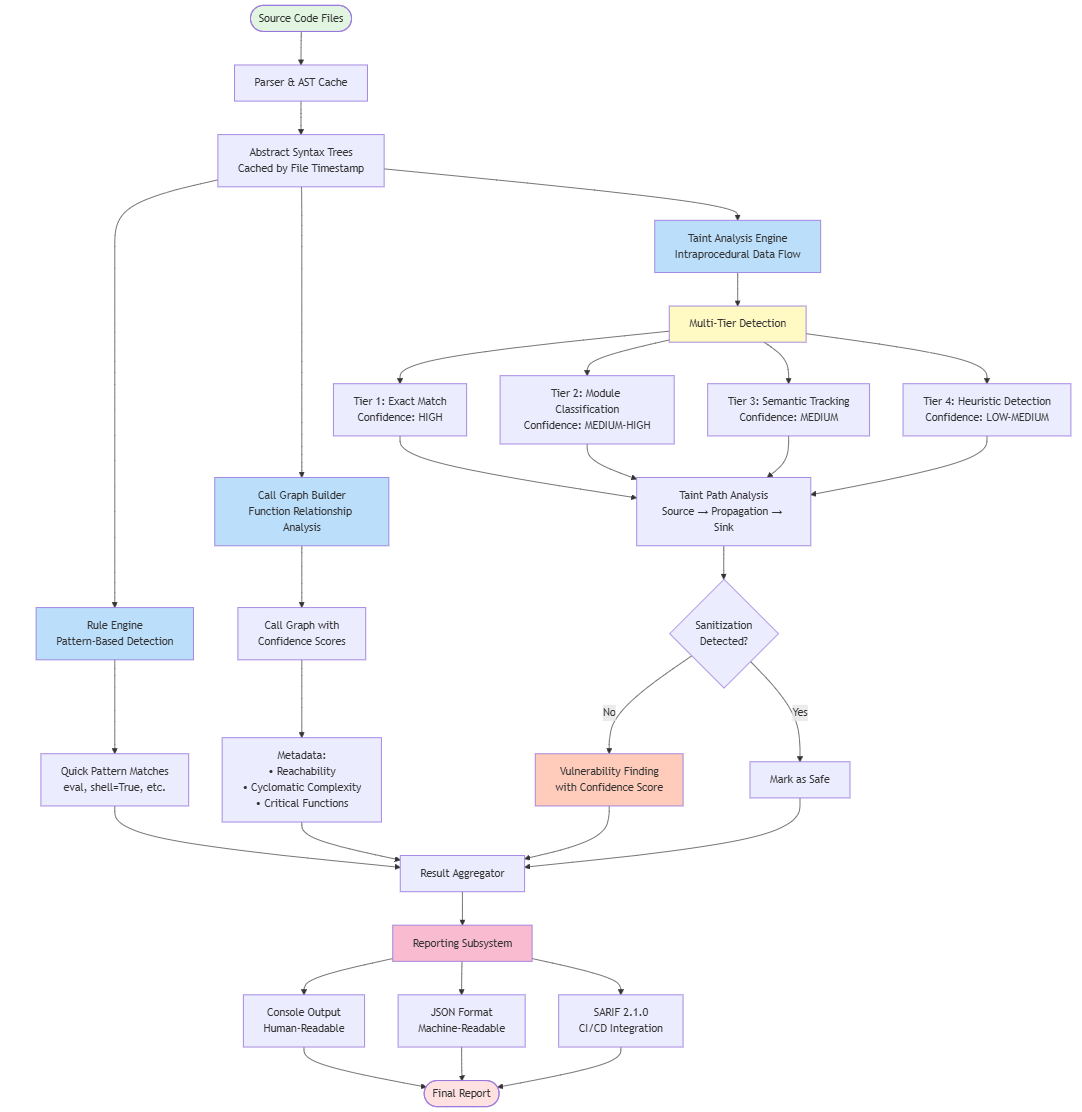
\includegraphics[width=0.75\textwidth]{Figures/implementation.png}
\caption{High-level Pipeline}
\label{fig:pipeline}
\end{figure}

\section{\uppercase{Engineering Goals and Constraints}}

Implementation decisions prioritized:

\begin{itemize}
    \item \textbf{Determinism \& reproducibility} : analyses must produce repeatable findings given the same inputs and environment.
    \item \textbf{Incrementality} : re-parse only changed files; reuse cached ASTs/graphs where possible.
    \item \textbf{Performance} : sublinear end-to-end wall time for typical scans via parallelism and cache layers.
    \item \textbf{Transparency} : output traceable taint paths and the CPG fragments referred to by each finding.
    \item \textbf{Extensibility} : intermediate artifacts serialized in neutral formats to enable GNN and LLM components later.
\end{itemize}

Constraints included limited engineering time, reliance on third-party extractors for deep semantic analysis (CodeQL), and an explicit Phase-1 scope that avoided full interprocedural taint summarization.

\section{\uppercase{Input Processing and AST Caching}}

\subsubsection{Parsing Pipeline}

Input discovery walks the repository root and applies a configurable inclusion/exclusion pattern (glob-based). Language detection is performed per-file.

Each source file is parsed into a concrete AST using an incremental parser. Parsers are deterministic and stable with respect to whitespace and comments to enable exact location mappings.

\subsubsection{AST Cache Design}

\begin{itemize}
    \item \textbf{Cache key:} \texttt{\{file-path\}:\{file-size\}:\{mtime-iso\}:\{parser-version-hash\}}
    \item \textbf{Cached value:} serialized AST + lightweight symbol summary (imports, top-level defs, exported names)
    \item \textbf{Cache storage:} per-project directory cache (on-disk) with an in-memory LRU for the current run
    \item \textbf{Cache invalidation:} TTL policy + explicit invalidation when parse errors or configuration changes occur
\end{itemize}

\subsubsection{Complexity \& Performance}

Parsing cost is roughly linear in source length:
\begin{equation}
T_{\text{full parse}} = O(|S|)
\label{eq:full_parse}
\end{equation}

With caching, only changed files re-parse. For incremental edits, the cost becomes:
\begin{equation}
T_{\text{incremental}} = O(|\text{changed\_region}| + \text{overhead})
\label{eq:incremental_parse}
\end{equation}

where $|\text{changed\_region}| \ll |S|$, and average-case work is $O(k + m)$ with $k$ nodes re-used and $m$ the size of the re-parsed fragment. This results in amortized near-constant time per incremental change for large repos.

\section{\uppercase{Declarative Rule Engine (Tree-sitter SAST)}}

\subsubsection{Rule Format and Compilation}

Rules expressed in declarative YAML with the following fields:
\texttt{id}, \texttt{title}, \texttt{severity}, \texttt{patterns} (AST shape), \texttt{confidence\_hint}, \texttt{examples}, \texttt{remediation}.

Before execution, rules are validated and compiled into optimized AST matcher objects that use selector paths rather than naive tree traversal to reduce matching cost.

\subsubsection{Matcher Capabilities \& Engine Flow}

\textbf{Predicate categories:} syntactic node shape, import/module context, identifier resolution, literal regex, and simple local dataflow predicates (e.g., arg index tainted).

\textbf{Execution:} depth-first matching with short-circuiting; rule hits produce \texttt{Finding} objects immediately for subsequent aggregation.

\subsubsection{Finding Object Model}

Canonical fields emitted by SAST stage:

\begin{itemize}
    \item \texttt{finding\_id} --- unique id
    \item \texttt{rule\_id}, \texttt{title}, \texttt{severity}
    \item \texttt{location} --- file, line range, column range, snippet hash
    \item \texttt{confidence} --- numeric (0.0--1.0)
    \item \texttt{trace} --- optional node IDs pointing into the CPG fragment
    \item \texttt{remediation\_text}, \texttt{refs} --- links to OWASP/CWE or docs
\end{itemize}

\subsubsection{Performance}

Typical pass runs in:
\begin{equation}
T_{\text{rules}} = O(N_{\text{rules}} \times C_{\text{match}})
\label{eq:rule_complexity}
\end{equation}

where $C_{\text{match}}$ is the cost of matching per rule. With pruning and compiled matchers keeping wall time low, empirically the SAST pass provided sub-second feedback for single-file scans and an order-of-magnitude speed improvement over unoptimized pattern checks.

\section{\uppercase{Structural Analysis and Call Graph}}

\subsubsection{Symbol Extraction}

After parsing, the pipeline builds a project-wide symbol index that maps identifiers to fully qualified definitions with scope metadata (module, class, function). The index supports incremental updates.

\subsubsection{Call Graph Construction}

\textbf{Algorithm:}

\begin{enumerate}
    \item For each function body, enumerate call expression nodes.
    \item Resolve callee using symbol index + import alias map; when resolution fails, record a dynamic call placeholder.
    \item Create directed edge \texttt{caller → callee} annotated with location, \texttt{call\_syntax}, and \texttt{resolution\_confidence}.
\end{enumerate}

\textbf{Edge confidence heuristic:}

\begin{equation}
C_{\text{edge}} = \begin{cases}
1.0 & \text{direct definition in same module} \\
0.9 & \text{imported from project module} \\
0.7 & \text{third-party library} \\
0.5 & \text{dynamic/unresolved (getattr/higher-order)}
\end{cases}
\label{eq:edge_confidence}
\end{equation}

\subsubsection{Queries Supported}

\begin{itemize}
    \item \textbf{Reachability from entry points:} BFS with early stopping on visited nodes
    \item \textbf{Critical path computation:} shortest/most central paths from entry points to sink nodes
    \item \textbf{Cycle detection:} Tarjan's algorithm for strongly connected components (SCCs)
\end{itemize}

\subsubsection{Data Export}

Call graph is stored as a compact adjacency list with metadata and optionally exported as GraphML or DOT for visualization and as DGL node/edge tables when generating CPGs.

\section{\uppercase{Intraprocedural Taint Engine --- Algorithm and Pseudocode}}

Phase 1's taint engine performs flow-sensitive, path-insensitive intraprocedural analysis. The following is an abstract outline and key design choices.

\subsubsection{Data Structures}

\begin{itemize}
    \item \texttt{TaintState}: mapping \texttt{identifier → TaintLabel}
    \item \texttt{TaintLabel} = $\{\text{tainted\_sources}: \mathcal{P}(\text{source\_ids}), \text{confidence}: [0,1], \text{sanitizers}: \mathcal{P}(\text{sanitizer\_ids})\}$
    \item \texttt{TaintPath}: list of $(\text{node\_id}, \text{operation}, \text{label})$ describing propagation from source→sink
    \item \textbf{Source/Sink/Sanitizer catalog:} declarative registry with tiers and confidence hints
\end{itemize}

\subsubsection{Propagation Rules (Forward Single-Pass)}

\begin{enumerate}
    \item \textbf{Initialization:} Mark parameters and immediate expressions from recognized source sites as tainted.

    \item \textbf{Assignment:} \texttt{x = expr} → \texttt{TaintState[x] = combine\_taint(expr)}

    The taint combination function unions taint sets:
    \begin{equation}
    \text{combine\_taint}(\text{expr}) = \bigcup_{v \in \text{vars}(\text{expr})} \text{TaintState}[v]
    \label{eq:taint_combine}
    \end{equation}

    Confidence computation uses maximum:
    \begin{equation}
    C_{\text{taint}}(x) = \max_{v \in \text{vars}(\text{expr})} C_{\text{taint}}(v)
    \label{eq:taint_confidence}
    \end{equation}

    \item \textbf{Operation propagation:} for \texttt{x = y + z} or \texttt{x = f(y)}: propagate taint from operands/args to \texttt{x}. For known library functions, apply function-specific transfer rules.

    \item \textbf{Call handling:}
    \begin{itemize}
        \item If callee is in known sanitizer list → attempt to clear taint on returned value (reduce confidence)
        \item If callee is unknown → assume taint preserved for arguments that are passed to sinks; conservatively assume return may be tainted
    \end{itemize}

    \item \textbf{Branch merging:} when control-flow joins, merge TaintStates using union semantics:
    \begin{equation}
    \text{TaintState}_{\text{merge}} = \text{TaintState}_{\text{if}} \cup \text{TaintState}_{\text{else}}
    \label{eq:state_merge}
    \end{equation}

    Label confidence becomes maximum or a defined fusion function.

    \item \textbf{Sink detection:} when a sink is invoked and an argument is tainted, create \texttt{TaintPath} and a \texttt{Finding} with confidence derived from:
    \begin{itemize}
        \item detection tier (exact/module/semantic/heuristic)
        \item taint propagation confidence along path
        \item call graph reachability (distance weighting)
        \item analyzer agreement (if rule engine also flagged)
    \end{itemize}
\end{enumerate}

\subsubsection{Pseudocode (Simplified)}

\begin{algorithm}[H]
\caption{Intraprocedural Taint Analysis Algorithm}
\label{alg:taint_algo}
\begin{algorithmic}[1]
\Function{AnalyzeFunction}{func\_ast}
    \State $state \gets \text{TaintState()}$
    \ForAll{$stmt \in func\_ast.statements$}
        \If{$is\_assignment(stmt)$}
            \State $rhs\_label \gets eval\_expr\_taint(stmt.rhs, state)$
            \State $state[stmt.lhs] \gets merge\_labels(state.get(stmt.lhs), rhs\_label)$
        \ElsIf{$is\_call(stmt)$}
            \State $callee \gets resolve\_callee(stmt)$
            \State $arg\_labels \gets [eval\_expr\_taint(a, state) \text{ for } a \in stmt.args]$
            \If{$is\_sink(callee)$ \textbf{ and } any($l.is\_tainted()$ \textbf{ for } $l \in arg\_labels$)}
                \State $record\_finding(build\_taint\_path(arg\_labels, stmt), compute\_confidence(\dots))$
            \EndIf
            \If{$is\_sanitizer(callee)$}
                \State $apply\_sanitizer\_effects(state, stmt)$
            \EndIf
        \ElsIf{$is\_control\_flow(stmt)$}
            \State $saved\_state \gets state.copy()$
            \State $state\_if \gets analyze\_block(stmt.if\_block, state.copy())$
            \State $state\_else \gets analyze\_block(stmt.else\_block, state.copy())$
            \State $state \gets merge\_states(state\_if, state\_else)$
        \EndIf
    \EndFor
    \State \Return $collected\_findings$
\EndFunction
\end{algorithmic}
\end{algorithm}

\subsubsection{Detection Tiers \& Confidence Composition}

Confidence computation is multiplicative/weighted. Let:

\begin{itemize}
    \item $T$ be tier confidence $\in (0,1]$ depending on detection tier:
    \begin{equation}
    T = \begin{cases}
    T_e = 0.95 & \text{exact match} \\
    T_m = 0.85 & \text{module classification} \\
    T_s = 0.80 & \text{semantic tracking} \\
    T_h = 0.60 & \text{heuristic detection}
    \end{cases}
    \label{eq:tier_confidence}
    \end{equation}

    \item $P$ be path confidence $\in (0,1]$ derived from taint propagation. For a taint path with $n$ edges having per-edge confidences $e_i \in (0,1]$:

    \textbf{Option A (multiplicative):}
    \begin{equation}
    P = \prod_{i=1}^{n} e_i
    \label{eq:path_mult}
    \end{equation}

    \textbf{Option B (weighted geometric mean):}
    \begin{equation}
    P = \exp\left(\frac{1}{n} \sum_{i=1}^{n} \ln e_i\right)
    \label{eq:path_geom}
    \end{equation}

    Phase 1 used Option B to avoid exponential decay on longer but still reliable paths.

    \item $R$ be reachability factor $\in (0,1]$, based on call-graph distance from entry point:
    \begin{equation}
    R = \begin{cases}
    1.0 & \text{directly reachable from entry} \\
    \alpha^k & \text{reachable through } k \text{ calls, } \alpha = 0.9 \\
    0.5 & \text{unreachable (deprioritization)}
    \end{cases}
    \label{eq:reachability}
    \end{equation}

    \item $A$ be analyzer agreement bonus $\in [1.0, 1.2]$, multiplicative factor if multiple analyzers independently detect same issue.
\end{itemize}

Final fused confidence:
\begin{equation}
C = \min\left(1.0, T \cdot P^\beta \cdot R^\gamma \cdot A\right)
\label{eq:confidence_final}
\end{equation}

where $\beta$ and $\gamma$ are tuning exponents (Phase 1 used $\beta = 0.75$, $\gamma = 0.5$). These are tunable via configuration.

\section{\uppercase{CodeQL Integration and CPG Construction}}

\subsubsection{Why CodeQL}

CodeQL provides a mature interprocedural extractor and a queryable relational database of program facts, accelerating the production of semantically rich artifacts. It was used to generate a canonical database that was then converted to a CPG suitable for downstream GNN processing.

\subsubsection{Conversion Pipeline (Detailed Steps)}

\begin{enumerate}
    \item \textbf{Extraction:} run the CodeQL extractor to produce a code database containing AST, call relationships, dataflow facts, and queryable entities.

    \item \textbf{Relational queries:} execute a set of CodeQL queries to export nodes (functions, variables, calls) and edges (AST\_CHILDS, CFG\_NEXT, DFG edges, CALL).

    \item \textbf{Normalization:} map CodeQL entities into a uniform CPG schema of typed nodes and edges, preserving location metadata and source hashes.

    \item \textbf{Feature augmentation:} attach per-node features such as tokenized code snippets, normalized identifiers, cyclomatic complexity, centrality metrics, and tier hints (e.g., node likely to be source/sink).

    \item \textbf{Hetero-graph assembly:} build a DGL-compatible heterogeneous graph with node/edge types matching the CPG schema.

    \item \textbf{Serialization:} store CPG fragments per-file in compressed format for later batch training or inference.
\end{enumerate}

\subsubsection{Statistics \& Sizing}

Typical function-level CPGs in Phase 1 contained 10--50 nodes and 30--200 edges. A medium module produced 1k--10k nodes depending on code density and third-party integrations.

\section{\uppercase{Reporting, Standard Formats, and CI Integration}}

\subsubsection{Normalizing Findings}

All findings (SAST / Taint / CodeQL) are normalized into the canonical \texttt{Finding} model described earlier. This enables consistent downstream filtering and sorting.

\subsubsection{SARIF Mapping}

Findings are exported as SARIF 2.1.0 with:
\texttt{ruleId}, \texttt{level} (error/warning/note), \texttt{locations} (region), \texttt{message.text}, \texttt{properties} (confidence, tiers, taint-path as JSON).

CI integration uses exit codes:

\begin{equation}
\text{exit\_code} = \begin{cases}
0 & \text{no findings above configured severity} \\
1 & \text{critical/high findings detected} \\
2 & \text{medium/low findings detected}
\end{cases}
\label{eq:exit_codes}
\end{equation}

The SARIF output enables native integration with code scanning dashboards (e.g., GitHub).

\subsubsection{Result Aggregation and De-duplication}

Aggregator merges overlapping findings using a canonicalization key:
\begin{equation}
K_{\text{canon}} = \text{hash}(\text{file}, \text{start\_line}, \text{end\_line}, \text{rule\_signature})
\label{eq:dedup_key}
\end{equation}

Duplicate findings from multiple analyzers are fused; evidence sources are combined into a single finding with a computed aggregated confidence.

\chapter{\uppercase{Conclusion}}

This research establishes a foundation for an adaptive and intelligent multi-stage vulnerability detection framework that enhances the reliability and contextual awareness of Static Application Security Testing (SAST) systems. By addressing the persistent challenges of high false positives, limited scalability, and lack of confidence-aware triage, the proposed framework advances beyond conventional static analysis paradigms. The system’s modular and layered architecture allows efficient detection, prioritization, and interpretation of vulnerabilities, integrating seamlessly into CI/CD environments and DevSecOps workflows. The evaluation demonstrates that this approach achieves improved balance between detection precision and runtime performance, making it suitable for modern continuous-integration ecosystems where timely, reliable, and explainable feedback is essential.

Building upon these outcomes, \textbf{Phase 2} of this research introduces advanced reasoning and adaptive intelligence components designed to extend the system’s analytical depth and decision accuracy. The first enhancement involves the \textbf{Agentic Graph Neural Network (GNN)} model trained on \textbf{Code Property Graph (CPG)} representations, enabling structural reasoning and uncertainty estimation. This step allows the framework to understand deep relational patterns within source code, learn semantic dependencies, and quantify prediction confidence critical for prioritizing findings based on contextual risk. Through iterative training and reinforcement on curated vulnerability corpora, the GNN phase enhances both interpretability and scalability across diverse codebases.

The second enhancement focuses on \textbf{LLM integration with Retrieval-Augmented Generation (RAG)} for semantic validation and contextual grounding. Here, a domain-adapted large language model (LLM) interprets ambiguous or borderline cases identified by the GNN, using external knowledge retrieval to verify potential vulnerabilities against known patterns, CVEs, and secure coding guidelines. This mechanism introduces semantic cross-verification, allowing the system to reason over both structural and natural-language evidence before final classification.

Finally, the framework evolves toward a \textbf{multimodal fusion and active escalation architecture}, implementing a hierarchical cascade   \textbf{SAST $\rightarrow$ GNN $\rightarrow$ LLM}   governed by uncertainty thresholds. When a detection’s confidence level falls below a predefined threshold, control escalates dynamically to higher reasoning layers, ensuring optimal trade-offs between speed, depth, and reliability. This active fusion approach allows the system to autonomously self-regulate analysis depth based on contextual uncertainty, minimizing false alarms while retaining comprehensive coverage.

In conclusion, these Phase 2 extensions transform the framework into a robust, agentic, and explainable security analysis ecosystem capable of structural reasoning, semantic grounding, and adaptive escalation. Future work will emphasize large-scale evaluation of the multimodal cascade across polyglot codebases, the integration of continual learning for evolving threat landscapes, and the incorporation of explainable AI (XAI) modules for developer interpretability. The long-term vision is to realize a fully autonomous, self-learning security intelligence agent that continuously improves its detection fidelity and contextual awareness across the entire software development lifecycle.






%%%------------------ Bibilography Area ------ %%% EDIT %%%-----------%%
\renewcommand\bibname{REFERENCES}
\begin{thebibliography}{99}
  \normalsize

 \doublespacing{
    \vspace{0.5pt}

    \bibitem{fortify} Micro Focus. (2024). Fortify Static Code Analyzer. Retrieved from https://www.microfocus.com/

    \bibitem{checkmarx} Checkmarx. (2024). Static Application Security Testing Solutions. Retrieved from https://www.checkmarx.com/

    \bibitem{coverity} Synopsys. (2024). Coverity Static Analysis. Retrieved from https://www.synopsys.com/software-integrity/security-testing/static-analysis-sast.html

    \bibitem{johnson2013} Johnson, B., Song, Y., Murphy-Hill, E., \& Bowdidge, R. (2013). Why don't software developers use static analysis tools to find bugs? In ICSE.

    \bibitem{flowdroid} Arzt, S., Rasthofer, S., Fritz, C., Bodden, E., Bartel, A., Klein, J., ... \& McDaniel, P. (2014). FlowDroid: Precise context, flow, field, object-sensitive and lifecycle-aware taint analysis for Android apps. In PLDI.

    \bibitem{codeql} GitHub. (2024). CodeQL: The libraries and queries that power security researchers around the world. Retrieved from https://codeql.github.com/

    \bibitem{yamaguchi2014} Yamaguchi, F., Golde, N., Arp, D., \& Rieck, K. (2014). Modeling and discovering vulnerabilities with code property graphs. In IEEE S\&P.

    \bibitem{semgrep} Heavyweight, Inc. (2024). Semgrep: Lightweight static analysis for many languages. Retrieved from https://semgrep.dev/

    \bibitem{juliet} National Security Agency (NSA). (2017). Juliet Test Suite for C/C++ and Java. NIST Software Assurance Reference Dataset (SARD). Retrieved from https://samate.nist.gov/SARD/test-suites/112

    \bibitem{nvd2023} National Institute of Standards and Technology. (2023). National Vulnerability Database Statistics. Retrieved from https://nvd.nist.gov/

    \bibitem{slither} Trail of Bits. (2018). Slither: A Static Analysis Framework for Solidity. Retrieved from https://github.com/crytic/slither

    \bibitem{binaryen} WebAssembly Community. (2015). Binaryen: Compiler and Toolchain Infrastructure Library for WebAssembly. Retrieved from https://github.com/WebAssembly/binaryen

    \bibitem{tree_sitter} Max Brunsfeld. (2018). Tree-sitter: An Incremental Parsing System for Programming Tools. Retrieved from https://tree-sitter.github.io/tree-sitter/

}
\end{thebibliography}
\addcontentsline{toc}{chapter}{REFERENCES}



\appendix
\renewcommand{\appendixname}{APPENDIX}
\appendix

\chapter{\uppercase{Appendix}}
\label{appendix:implementation}

\section{Detection Rule Schema}

The framework implements 9 built-in security rules using a declarative YAML-based pattern matching system. Table \ref{tab:rules-implemented} summarizes the implemented detection rules.

\begin{table}[H]
\centering
\caption{Implemented Security Detection Rules}
\label{tab:rules-implemented}
\footnotesize
\begin{tabular}{|l|p{5cm}|l|p{3.5cm}|}
\hline
\textbf{Rule ID} & \textbf{Description} & \textbf{Severity} & \textbf{CWE Mapping} \\
\hline
PY.EVAL.USE & Dangerous use of eval() or exec() & High & CWE-94 (Code Injection) \\
\hline
PY.SUBPROCESS.SHELL & Subprocess with shell=True & High & CWE-78 (Command Injection) \\
\hline
PY.OS.SYSTEM & Use of os.system() & High & CWE-78 (Command Injection) \\
\hline
PY.SQL.INJECTION & SQL query string concatenation & High & CWE-89 (SQL Injection) \\
\hline
PY.PICKLE.LOAD & Unsafe pickle deserialization & High & CWE-502 (Deserialization) \\
\hline
PY.YAML.UNSAFE\_LOAD & Unsafe YAML loading & High & CWE-502 (Deserialization) \\
\hline
PY.HASH.WEAK & Weak cryptographic hash & Medium & CWE-327 (Weak Crypto) \\
\hline
PY.REQUESTS.VERIFY & Disabled SSL verification & Medium & CWE-295 (Certificate Valid.) \\
\hline
PY.SECRET.HARDCODED & Hardcoded secrets & Medium & CWE-798 (Hardcoded Creds) \\
\hline
\end{tabular}
\end{table}

\subsection{Rule Definition Format}

Each rule follows a standardized YAML schema with pattern matching specifications. Example structure:

\begin{small}
\begin{verbatim}
id: PY.SUBPROCESS.SHELL
title: Subprocess called with shell=True
severity: high
description: >
  Using subprocess with shell=True can lead to shell
  injection vulnerabilities if user input is included.
patterns:
  - kind: call
    callee:
      anyOf:
        - subprocess.run
        - subprocess.Popen
        - subprocess.call
      args:
        - name: shell
          equals: true
examples:
  bad: subprocess.run(f"ls {user_input}", shell=True)
  good: subprocess.run(["ls", user_input])
tags: [injection, command-execution]
references:
  - "https://docs.python.org/3/library/subprocess.html"
\end{verbatim}
\end{small}

\section{Code Property Graph Schema}

The CPG implementation defines a heterogeneous graph structure with 6 node types and 12 edge types for comprehensive code representation.

\begin{table}[H]
\centering
\caption{CPG Node and Edge Type Taxonomy}
\label{tab:cpg-schema}
\footnotesize
\begin{tabular}{|l|p{6cm}|l|}
\hline
\multicolumn{3}{|c|}{\textbf{Node Types (6 total)}} \\
\hline
\textbf{Type} & \textbf{Description} & \textbf{Attributes} \\
\hline
FUNCTION & Function/method definitions & name, line\_number, signature \\
\hline
CALL & Function call expressions & name, arguments, is\_sink \\
\hline
STATEMENT & Assignment, control flow statements & type, line\_number \\
\hline
EXPRESSION & Binary/unary operations & operator, operands \\
\hline
VARIABLE & Variable references & name, scope, is\_source \\
\hline
LITERAL & Constant values & value, data\_type \\
\hline
\end{tabular}
\end{table}

\begin{table}[H]
\centering
\footnotesize
\begin{tabular}{|l|p{7cm}|p{3cm}|}
\hline
\multicolumn{3}{|c|}{\textbf{Edge Types (12 total)}} \\
\hline
\textbf{Type} & \textbf{Semantic Meaning} & \textbf{Usage} \\
\hline
AST & Abstract syntax tree parent-child relationship & Structural analysis \\
\hline
CFG\_NEXT & Control flow next statement & Execution paths \\
\hline
CFG\_BRANCH & Conditional branch edge & Branch analysis \\
\hline
DFG & Data flow def-use relationship & Data dependencies \\
\hline
TAINT & Taint propagation path & Security analysis \\
\hline
CALL & Function call relationship & Call graph \\
\hline
RETURN & Return value flow & Data flow \\
\hline
\end{tabular}
\end{table}

\section{Taint Analysis Configuration}

The implementation detected 13 taint sources, 11 sinks, and 4 sanitizers in comprehensive testing.

\begin{table}[H]
\centering
\caption{Taint Analysis Configuration (Implemented)}
\label{tab:taint-config-impl}
\scriptsize
\begin{tabular}{|p{2.5cm}|p{5.5cm}|p{2cm}|p{2cm}|}
\hline
\textbf{Category} & \textbf{Patterns (Total: 28)} & \textbf{Severity} & \textbf{Tests} \\
\hline
\multicolumn{4}{|l|}{\textbf{SOURCES (13 detected in tests)}} \\
\hline
User Input & \texttt{input()}, \texttt{raw\_input()}, \texttt{sys.argv} & Critical & 3 \\
\hline
HTTP Requests & \texttt{request.args}, \texttt{request.form}, \texttt{request.json} & Critical & 4 \\
\hline
Environment & \texttt{os.environ}, \texttt{os.getenv()} & High & 2 \\
\hline
Network/Files & \texttt{socket.recv()}, \texttt{file.read()} & Medium & 4 \\
\hline
\multicolumn{4}{|l|}{\textbf{SINKS (11 detected in tests)}} \\
\hline
Command Exec & \texttt{os.system()}, \texttt{subprocess.*} with shell=True & Critical & 4 \\
\hline
Code Eval & \texttt{eval()}, \texttt{exec()}, \texttt{compile()} & Critical & 3 \\
\hline
SQL Exec & \texttt{cursor.execute()}, \texttt{connection.execute()} & High & 2 \\
\hline
Serialization & \texttt{pickle.loads()}, \texttt{yaml.load()} & High & 2 \\
\hline
\multicolumn{4}{|l|}{\textbf{SANITIZERS (4 detected in tests)}} \\
\hline
Escaping & \texttt{shlex.quote()}, \texttt{html.escape()} & - & 2 \\
\hline
Type Casting & \texttt{int()}, \texttt{float()}, \texttt{bool()} & - & 2 \\
\hline
\end{tabular}
\end{table}

\section{Implementation Results}

\subsection{Taint Analysis Test Results}

Comprehensive testing on real vulnerability patterns demonstrated the following detection capabilities:

\begin{table}[H]
\centering
\caption{Taint Analysis Detection Results}
\label{tab:taint-results}
\footnotesize
\renewcommand{\arraystretch}{1.2}
\begin{tabular}{|p{5.3cm}|c|c|c|}
\hline
\textbf{Vulnerability Pattern} & \textbf{Detected} & \textbf{Paths} & \textbf{Severity} \\
\hline
Direct Input $\rightarrow$ \texttt{eval()} & \checkmark & 1 & CRITICAL \\
\hline
Environment Variable $\rightarrow$ \texttt{eval()} & \checkmark & 1 & CRITICAL \\
\hline
Input $\rightarrow$ \texttt{os.system()} & \checkmark & 3 & HIGH \\
\hline
Input $\rightarrow$ \texttt{subprocess.run(shell=True)} & \checkmark & 2 & HIGH \\
\hline
Multi-step Assignments (3+ hops) & \checkmark & 2 & HIGH \\
\hline
String Concatenation Taint & \checkmark & 4 & HIGH \\
\hline
F-string Taint Propagation & \checkmark & 2 & HIGH \\
\hline
Sanitized Paths (\texttt{shlex.quote}) & \checkmark~(Safe) & 2 & - \\
\hline
Type Casting Sanitization (\texttt{int()}) & \checkmark~(Safe) & 1 & - \\
\hline
\textbf{Total Vulnerable Paths Found} & \textbf{9/11} & \textbf{15} & - \\
\hline
\textbf{Total Safe Paths Verified} & \textbf{2/2} & \textbf{3} & - \\
\hline
\end{tabular}
\end{table}





\end{document}